
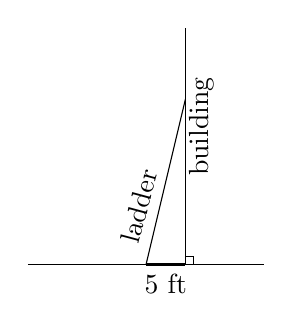
\begin{tikzpicture}
\draw[very thin](0,0)--(3,0);
\draw(2,0)--(2,3);
\draw(1.5,0)--(2,2.1);
\draw(1.8,1.26)node[anchor=south east, rotate=75]{ladder};
\draw[very thick](1.5,0)--(2,0);
\draw(1.75,0)node[anchor=north]{5 ft};
\draw(2.2,1)node[anchor=west, rotate = 90]{building};
\draw(2,.1)rectangle(2.1,0);
\end{tikzpicture}

A ladder is leaning up against a building on level ground.
The foot of the ladder is $5$ feet from the building, and
the ladder leans with a slope of $4.2$.  How far from the
ground, in feet, is the top of the ladder?



\ifsat
	\begin{enumerate}[label=\Alph*)]
		\item $0.84$
		\item $1.19$
		\item $9.2$
		\item $21$%
	\end{enumerate}
\else
\fi

\ifacteven
	\begin{enumerate}[label=\textbf{\Alph*.},itemsep=\fill,align=left]
		\setcounter{enumii}{5}
		\item $0.84$
		\item $1.19$
		\item $9.2$
		\addtocounter{enumii}{1}
		\item $21$%
		\item $47$
	\end{enumerate}
\else
\fi

\ifactodd
	\begin{enumerate}[label=\textbf{\Alph*.},itemsep=\fill,align=left]
		\item $0.84$
		\item $1.19$
		\item $9.2$
		\item $21$%
		\item $47$
	\end{enumerate}
\else
\fi

\ifgridin
 $21$%

\else
\fi

